% !TeX spellcheck = en_GB
\documentclass[12pt,landscape]{article}
\usepackage[a3paper]{geometry}
\usepackage{graphicx}
\usepackage{pdfpages}
\usepackage{wrapfig}
\usepackage{apacite}

\title{Designing A Water Tower}
\author{Lachlan Knell}
\begin{document}
\maketitle

\section{Introduction}
The Queensland Water alliance requires a new design for a water tower in Western Queensland. It will be constructed and transported to many locations, and requires that it be made of as little materials as possible. It must also be easy to mass produce and transport parts for.


\begin{wrapfigure}[0]{r}{0.3\textwidth}
	\centering
	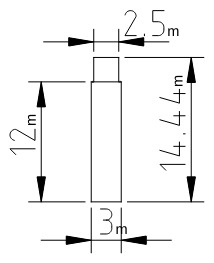
\includegraphics[trim={0 0cm 0 0cm},clip,scale=0.75]{WaterTower.jpg}
	\caption{\label{fig:BigWaterTower}Full-Size Specifications for the water tower}
\end{wrapfigure}

\vspace{5mm}

The task is to design the water tower adhering to the requirements as set by the Queensland Water Alliance, The tower is required to abide by these specific specifications:
\begin{itemize}
	\item Support A 12,000L Water tank with a 2.5 m diameter 
	\item Constructed to a height of 12 m
	\item Have a maximum base of 3x3 m 

\end{itemize}

\vspace{5mm}
In addition the prototype is required to be constructed to these specifications:
\begin{itemize}
	\item Supports 40kg of weight,
	\item It must use less than 10 lengths of 915x6x6mm Balsa Wood,
	\item Built to a 1:30 scale of the intended final design 
\end{itemize}


\section{Research}

There are many potential designs for vertical structures, and it is imperative that the most efficient design be constructed from the materials given. It should use as little material as possible, while retaining sufficient capability for reducing the forces present on the tower. 

\subsection{Mechanics}
Water Towers have to withstand significant forces from extreme weight contained within the water tower, often an entire days worth of water for a community (Green, 2022) 


- Research
- Engineering technology 
Triangles are good for distributing force when pushed on its points, making it good for designing objects under strain.
- Mechanics 
The tower needs to support high amounts of compressive and tensile forces in the individual braces, Cross braces will also need to be implemented to reduce the deflective forces.
- Materials
Water towers are required to be built of non-porous (materials that don’t let water through); They also require materials that don’t rust, often using steel and other metals.

However the task requires that the prototypes be built of balsa wood due to its portability and ability to manipulate. 
Balsa wood is also good due to it having a tensile strength of 1MPa



- Analysis

- Mathematics
- Calculating material
- Calculating average density of pieces
- Calculating predicted mass

- Simulator and drawn designs

- Success criteria

Synthesis and evaluation 
- Evaluate design
Evaluation and success criteria
Recommendations

Communication 
Captioning images
Referencing properly

\bibliography{ref.bib}
\bibliographystyle{apacite}
\end{document}
